\chapter[Hyperparameters]{Hyperparameters}
\label{ch:Hyperparameters}

As stated by Li \textit{et al.} in \cite{Li2017}, "performance of machine learning algorithms depends critically on identifying a good set of hyperparameters". Hyperparameter tuning is a topic often discussed in literature describing any combination of machine learning algorithms. Adequate values set for hyperparameters will massively influence training of a model, be it in terms of processing time, as well as the actual robustness of the model in question. 

\section{Introduction}\label{sec:page-layout}
\subsection{Defining Hyperparameters}\label{sec:headings}\index{headings}
Hyperparameters are variables which are initialised before a machine learning model undergoes training. The general representation is as a vector, with common examples of hyperparameters including the learning rate of a model, regularization coefficients, and kernel parameters. Considering the learning rate, an improperly set value will greatly influence the training potential of a regression model or neural network. Extremely high learning rate values may render a system volatile, causing weight/parameter values to fluctuate very easily, whilst lower values may inhibit learning capabilities. Similarly, altering the regularization coefficient for a Support Vector Machine (SVM) may greatly affect the shape of its decision boundary.


\section{Approaches for Hyperparameter Optimization}
Owing to the necessity of optimal hyperparameter values in machine learning problems, various works of literature are dedicated solely to their optimization. During the past decade, methods have been refined and applied in a large number of model methods. The sections below will go through a number of these approaches found in published works.
\subsection{Gradient-Based Hyperparameter Optimization}
 A particular project by  Sathiya \textit{et al.}\cite{SathiyaKeerthi2006} investigates hyperparameter values in SVMs and Bayesian models. In this system, the variables $C$ and $\gamma$ are considered. C is the regularization coefficient, influencing how leniently the SVM hyperplane classifies observations. $\gamma$ defines the influence of points on the variance of a model.  Experiments in this study showed that performance of the SVM varied considerably as a function of hyperparameter values. Gradient-based optimization techniques were used, computing the slope of a performance validation function with respect to the vector $h$ of hyperparameters. The gradient-based system described allowed for a fast method to determine optimal sets of hyperparameters, which outperformed a \textit{grid search} method even for models with solely 2 hyperparameters.


\subsection{Hyperparameter Optimization Through Adaptive Resource Allocation}
 As stated by Li \textit{et al.} in a more recently published paper\cite{Li2017}, the interaction between hyperparameters themselves is often not well understood. Generally, the main point of interest in a system is how the hyperparameters influence its performance, rather than how they affect each other as one configuration. This leads to brute force methods being used, such as the grid search method mentioned above, and random searching. Whilst these methods may be used to find good values of hyperparameters, they will more than likely result in suboptimal settings, especially for larger scale models. Bayesian techniques aim to optimize hyperparameter configurations by selecting them adaptively, beating out brute-force methods. Adaptive resource allocation is one such method which is used for selection. Strong hyperparameter configurations bearing positive results are provided more resources, such as an increased amount of training attributes. Other reward mechanisms include a larger number of features and epochs being provided. Other settings with less promising results may be discarded or allotted an inferior amount of resources. 

\subsection{Bandit-Based Approach in Conjunction with Adaptive Allocation}
 The HYPERBAND system was constructed by the same authors as above. It attempts to evaluate randomly-sampled hyperparameter configurations by adaptively assigning the corresponding amount of resources according to validation losses. This is termed a bandit-based approach since the project makes use of 'infinite armed bandits' in its implementation. Bandit arms represent mean-level reward distributions from particular experiments. The reward budget of each arm is essential for selection of the best distributions.  As detailed by Wang \textit{et al.} in \cite{Wang2009}, multi-armed bandit problems focus on \textit{exploration} vs. \textit{exploitation}. Arms can be `exploited', meaning that they performed well and may be selected for their respective task. Exploration may entail pulling entirely new arms, or pulling already discovered ones of interest. Scoping back to the HYPERBAND paper, the focus is on exploration infinite-armed bandit problems, selecting arms within the top reward percentiles for hyperparameter optimization.


\section{Scenario: Hyperparameter Tuning for Gradient Descent}
This scenario will look into a practical example of how hyperparameter values affect the performance of a gradient descent algorithm. Consider the following setup with cost function:

\begin{eqnarray}
y = 4x^{2} - 2x - 1 \\
dy/{dx} = 8x-2
\end{eqnarray}

\noindent The objective of gradient descent algorithms is to minimize a function. Mathematically, this implies that the algorithm will cycle through different values of $x$ until a minimum value of y is obtained, generally to a predefined precision. This process may be represented by the decrease in magnitude of the gradient of the function, hence the inclusion of the first derivative. The primary hyperparameter to be optimized in this case will be $\alpha$, representing the learning rate. As previously stated, the learning rate will affect the capability of the system to evolve. Values are calculated as follows for each iteration:

\begin{eqnarray}
x_{new} = x_{i} - \alpha(dy/{dx_{i}}) \\
y_{new} = (4(x_{new}^{2}) - 2x_{new} - 1  
\end{eqnarray}

\noindent  Another important parameter in this setup is $x_{0}$, which is the initial x-value to be used as an estimate for the minimum point. The following plot shows the algorithm with an $\alpha$ of $0.0001$:

 \begin{figure}
	\begin{center}
		\centering{{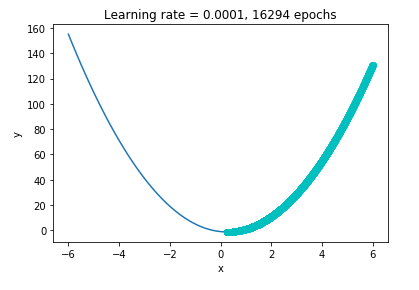
\includegraphics[width=0.82\textwidth]{graphics/hyperparameters/Grad_Desc_LR0001}}}
	\end{center}
	\caption{Plot of gradient descent with $\alpha = 0.0001$} \label{f:LR0001}
\end{figure}

\noindent In the figure above, $x_{0}$ has been set to 6 to simulate a poor estimate for the minimum x value. It can be observed from this plot, that the algorithm took 16294 iterations to converge on the local minima. The below plots will show the same setup with $\alpha$ values of 0.005 and 0.1: \clearpage

 \begin{figure}
	\begin{center}
		\centering{{\includegraphics[width=0.8\textwidth]{graphics/hyperparameters/Grad_Desc_LR005}}}
	\end{center}
	\caption{Plot of gradient descent with $\alpha = 0.005$} \label{f:LR005}
\end{figure}


 \begin{figure}
	\begin{center}
		\centering{\scalebox{0.76}{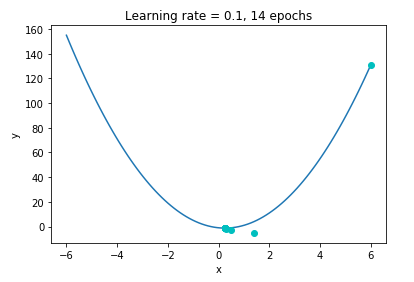
\includegraphics{graphics/hyperparameters/Grad_Desc_LR01}}}
	\end{center}
	\caption{Plot of gradient descent with $\alpha = 0.1$} \label{f:LR01}
\end{figure}

\noindent Increasing the learning rate will allow for the algorithm to converge much faster in this case. It is noteworthy that this was a straightforward example for visualization purposes. Learning models will generally be composed of various hyperparameters, and even variables such as the learning rate have certain intricacies, as discussed briefly above.


 


